\documentclass[a4paper, 12pt]{article}

% --- PAKIETY ---
\usepackage[utf8]{inputenc}
\usepackage[T1]{fontenc}
\usepackage[polish]{babel}
\usepackage{geometry}
\usepackage{xcolor}
\usepackage{hyperref}
\usepackage{graphicx}
\usepackage{fancyhdr}
\usepackage{beramono}

% --- NOWE PAKIETY DO OKIENEK TERMINALA ---
\usepackage{minted} % Do kolorowania składni (wymaga -shell-escape)
\usepackage[most]{tcolorbox}
\tcbuselibrary{minted,breakable} % Załadowanie bibliotek tcolorbox

% --- USTAWIENIA STRONY ---
\geometry{a4paper, left=2.5cm, right=2.5cm, top=2.5cm, bottom=2.5cm}
\definecolor{titlebg}{HTML}{4A90E2}

% --- USTAWIENIA HYPERLINKÓW ---
\hypersetup{
    colorlinks=true,
    linkcolor=titlebg,
    urlcolor=titlebg,
    citecolor=titlebg,
}

% --- NAGŁÓWEK I STOPKA ---
\pagestyle{fancy}
\fancyhf{}
\fancyhead[L]{Maszyna wirtualna z systemem Ubuntu}
\fancyfoot[C]{\thepage}
\renewcommand{\headrulewidth}{0.4pt}
\renewcommand{\footrulewidth}{0.4pt}

% --- STYLE DLA RAMEK TCOLORBOX ---
\newtcolorbox{definitionbox}[1]{
    colback=black!5, colframe=titlebg, fonttitle=\bfseries, coltitle=white,
    colbacktitle=titlebg, title=#1, boxrule=1pt, arc=4mm,
    bottomrule=0.5pt, toprule=0.5pt, breakable
}

\newtcolorbox{importantbox}[1]{
    colback=yellow!10, colframe=orange!80!black, fonttitle=\bfseries,
    title=#1, boxrule=1pt, arc=2mm, breakable
}

% --- STRONA TYTUŁOWA ---
\title{\bfseries Instrukcja instalacji oraz konfiguracji maszyny wirtualnej z systemem Ubuntu}
\author{Szymon Selwat}
\date{22 stycznia 2026}

% --- POCZĄTEK DOKUMENTU ---
\begin{document}

\maketitle
\thispagestyle{empty}
\newpage

\tableofcontents
\newpage

\section{Pobieranie i instalacja VirtualBox}
\subsection{Pobieranie instalatora VirtualBox}
Przejdź na stronę VirtualBox \href{https://www.virtualbox.org/}{https://www.virtualbox.org/}

\begin{figure}[H]
\centering
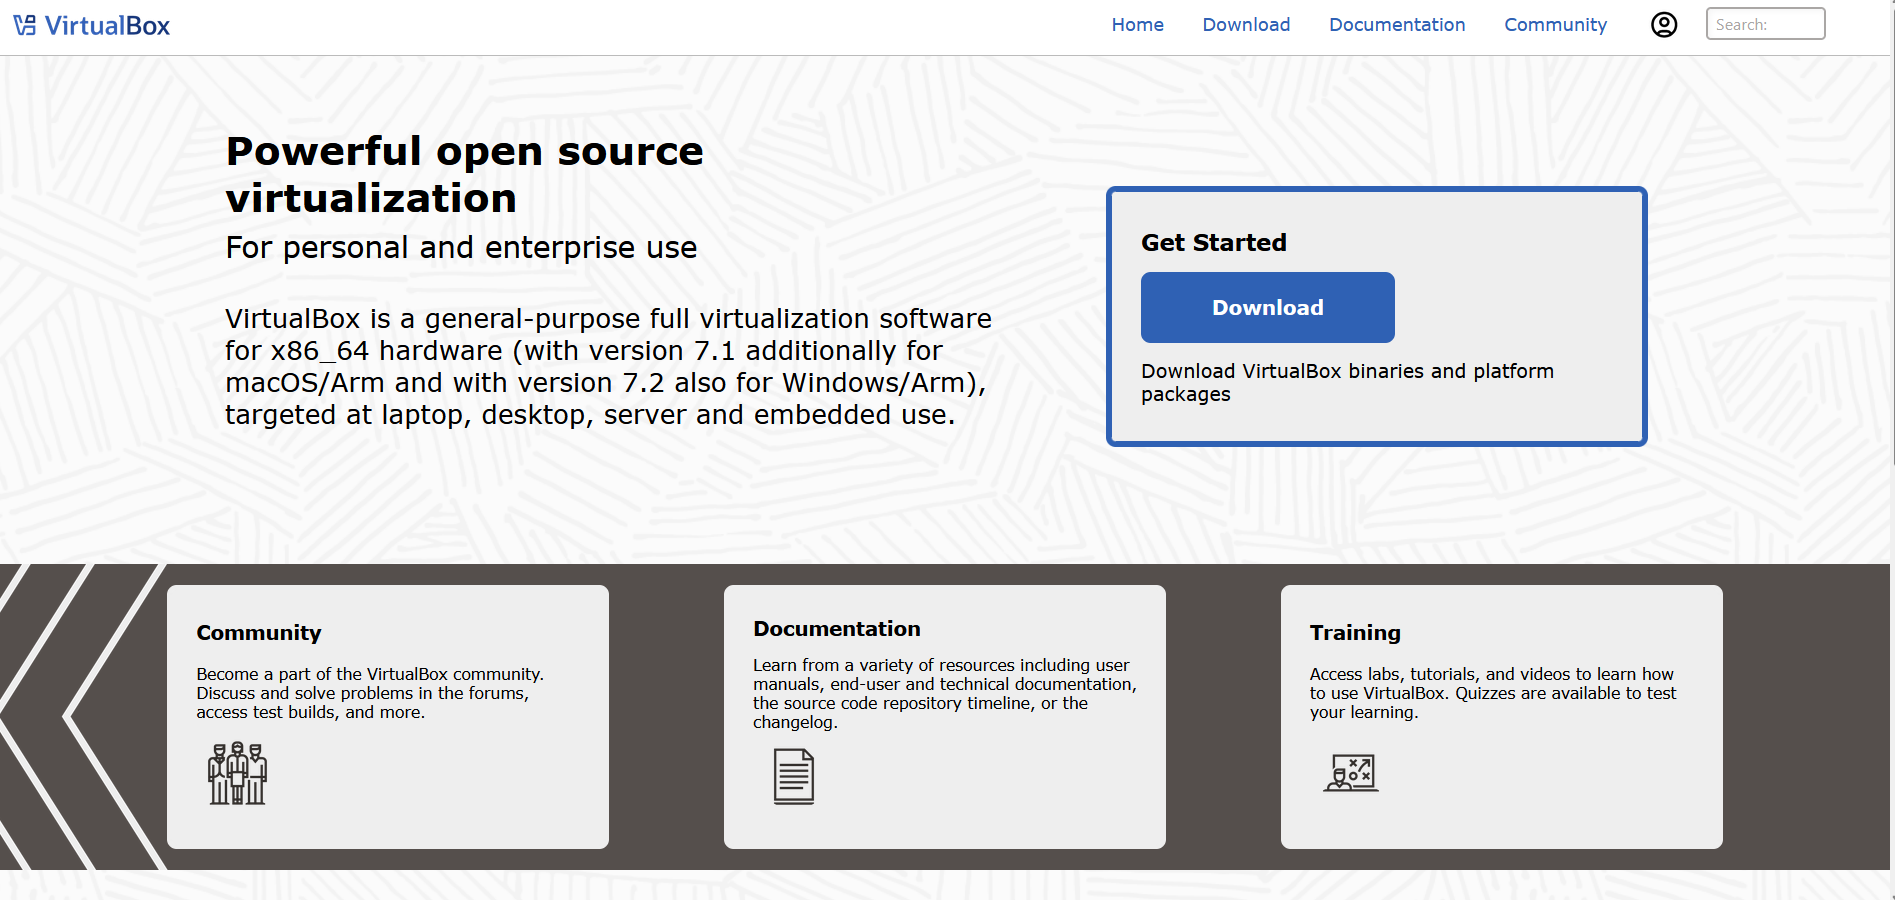
\includegraphics[width=0.8\textwidth]{screenshots/virtualbox1.png}
\end{figure}

Wejdź w zakładkę \textbf{Downloads} i wybierz wersję programu dla swojego systemu operacyjnego \textit{(Windows, macOS, Linux)}.

\begin{figure}[H]
\centering
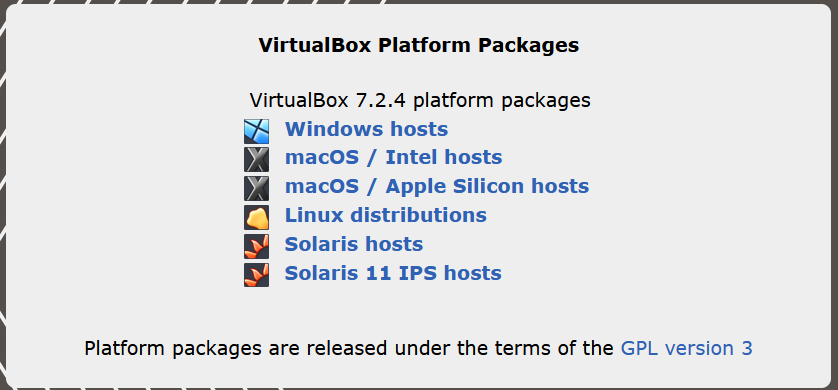
\includegraphics[width=0.8\textwidth]{screenshots/virtualbox2.png}
\end{figure}

Pobierz instalator i uruchom go.

\subsection{Instalowanie VirtualBox}
\begin{figure}[H]
\centering
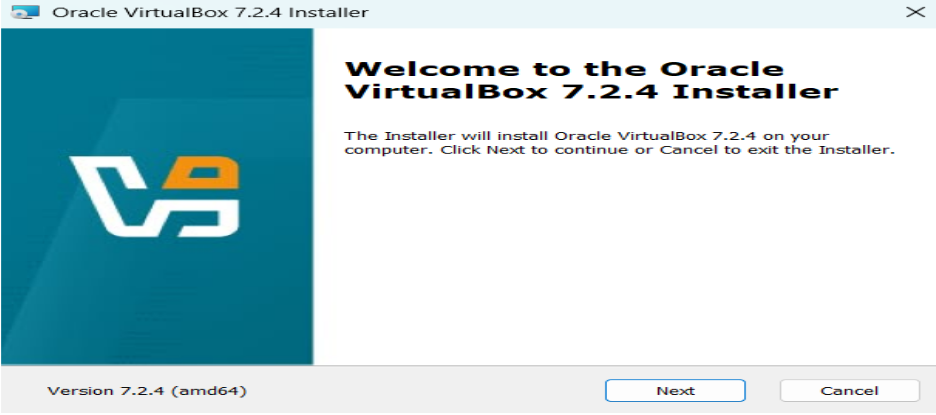
\includegraphics[width=0.8\textwidth]{screenshots/virtualbox3.png}
\end{figure}

Przejdź przez instalator zgodnie z instrukcjami wyświetlanymi na ekranie.

\begin{figure}[H]
\centering
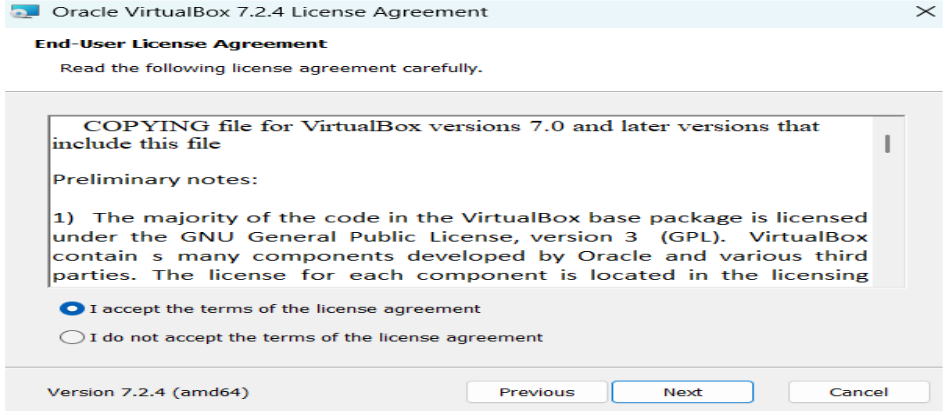
\includegraphics[width=0.8\textwidth]{screenshots/virtualbox4.png}
\end{figure}

\begin{figure}[H]
\centering
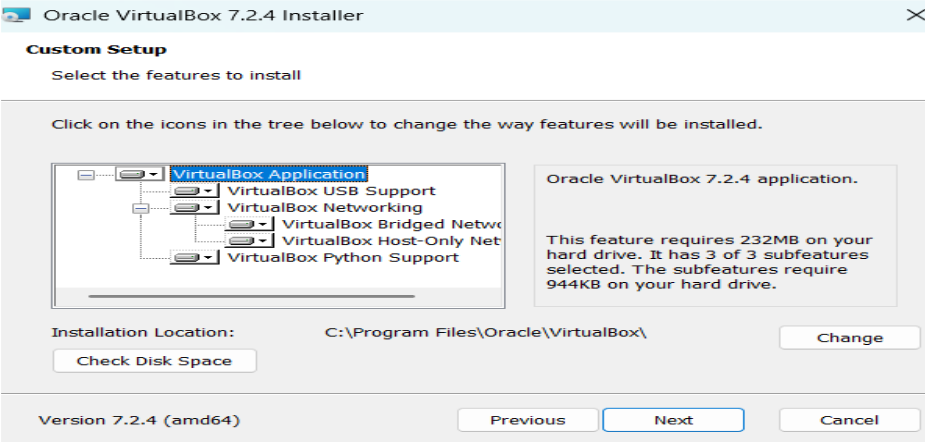
\includegraphics[width=0.8\textwidth]{screenshots/virtualbox5.png}
\end{figure}

Wybierz miejsce na dysku, w którym ma zostać zainstalowana Maszyna Wirtualna. \textit{Najlepiej zostawić opcję domyślną.}

\begin{figure}[H]
\centering
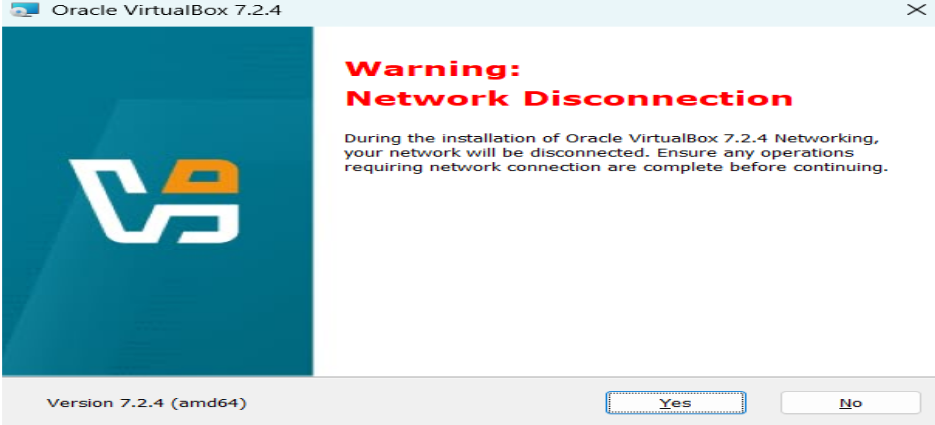
\includegraphics[width=0.8\textwidth]{screenshots/virtualbox6.png}
\end{figure}

Jeżeli wyskoczy komunikat taki jak powyżej, można to zignorować i przejść dalej poprzez kliknięcie \texttt{Yes}.

\begin{figure}[H]
\centering
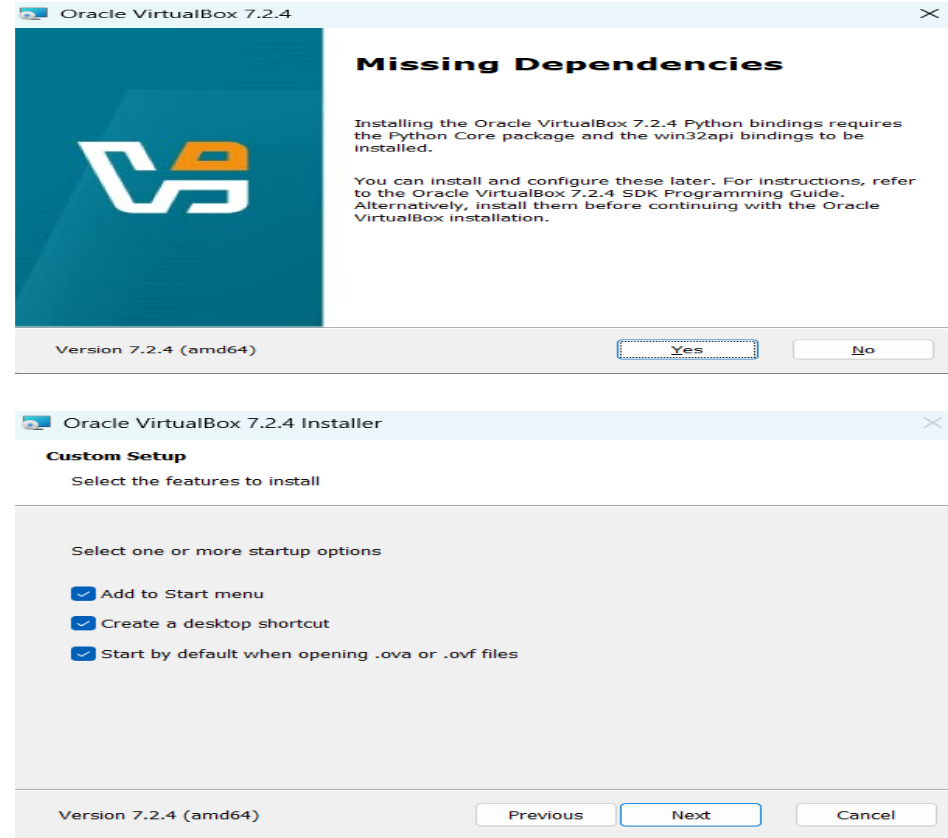
\includegraphics[width=0.8\textwidth]{screenshots/virtualbox7.png}
\end{figure}

\begin{figure}[H]
\centering
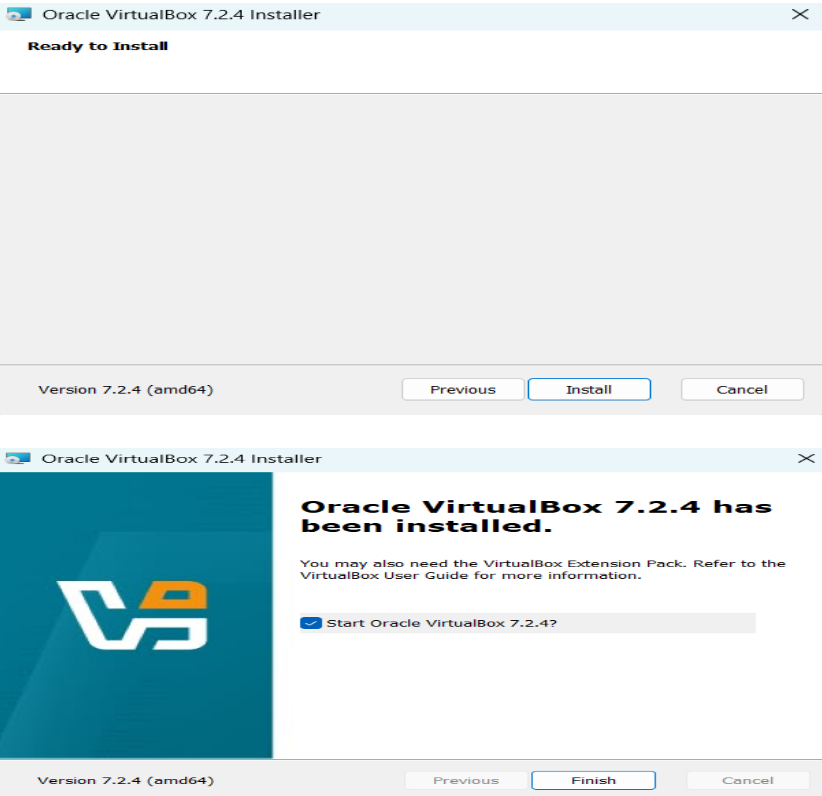
\includegraphics[width=0.8\textwidth]{screenshots/virtualbox8.png}
\end{figure}

Po skończonej instalacji i kliknięciu \texttt{Finish} oraz zaznaczeniu opcji \texttt{Start Oracle VirtualBox} nasz program powinien się uruchomić i pokazać następujący ekran:

\begin{figure}[H]
\centering
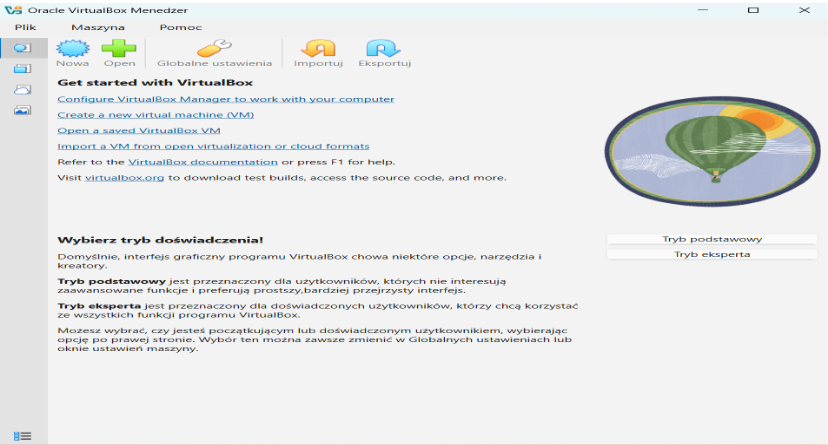
\includegraphics[width=0.8\textwidth]{screenshots/virtualbox9.png}
\end{figure}
\newpage

\section{Pobieranie pliku systemowego Ubuntu}
Przejdź na stronę Ubuntu \href{https://www.ubuntu.com/}{https://www.ubuntu.com/} i kliknij w zakładkę \texttt{Download Ubuntu}, a następnie \texttt{Download Ubuntu Desktop}.

\begin{figure}[H]
\centering
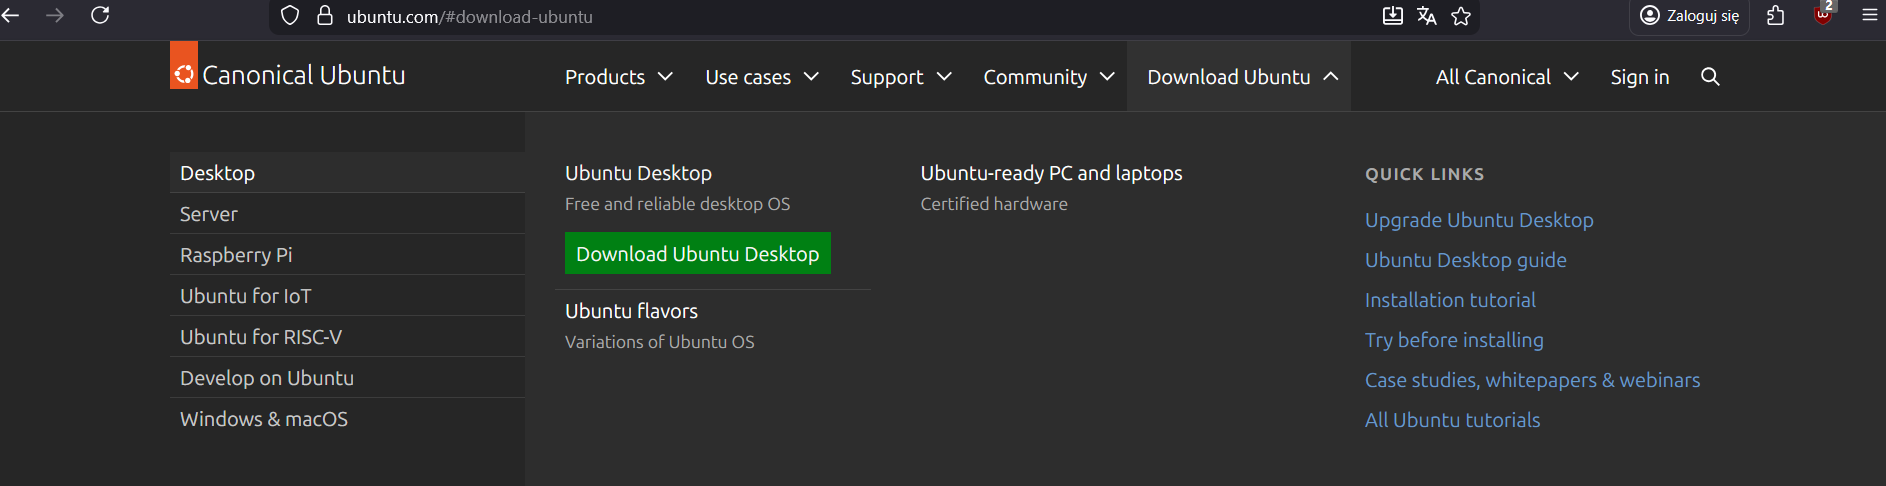
\includegraphics[width=0.8\textwidth]{screenshots/ubuntu1.png}
\end{figure}

Następnie znajdź sekcję z napisem \texttt{Ubuntu (...) LTS} \textit{( (...) oznacza numer najnowszej wersji, w moim przypadku 24.04.3)} i naciśnij przycisk \texttt{Download}.

\begin{figure}[H]
\centering
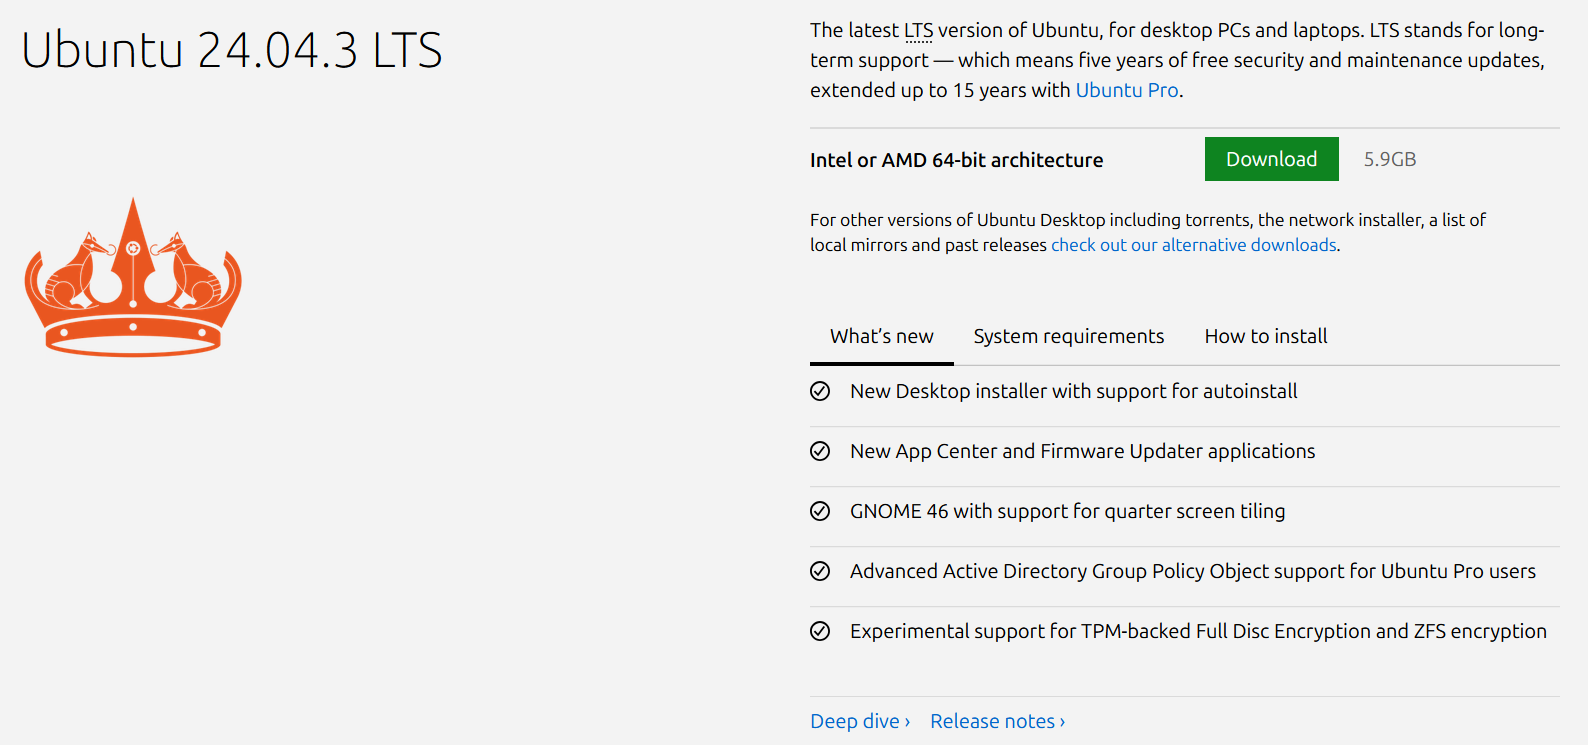
\includegraphics[width=0.8\textwidth]{screenshots/ubuntu2.png}
\end{figure}

Poczekaj aż pobieranie się zakończy.
\newpage

\section{Przygotowanie Maszyny Wirtualnej}
\subsection{"Postawienie" Maszyny Wirtualnej na nogi}
Uruchom \texttt{Oracle VirtualBox} i kliknij przycisk \texttt{Nowa} w lewym górnym rogu, żeby rozpocząć konfigurację twojej Maszyny Wirtualnej.

\begin{figure}[H]
\centering
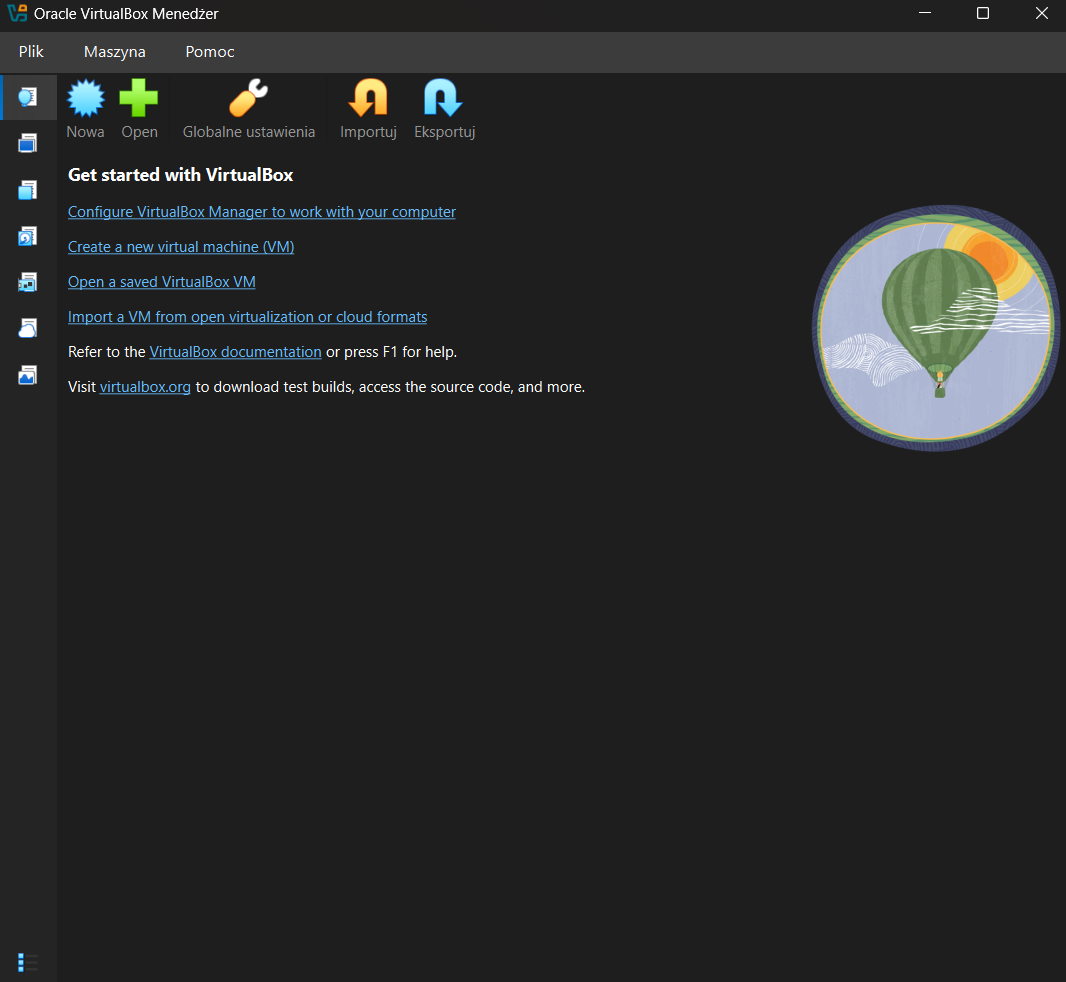
\includegraphics[width=0.7\textwidth]{screenshots/install01.png}
\end{figure}

Następnie pojawi się takie okno:
\begin{figure}[H]
\centering
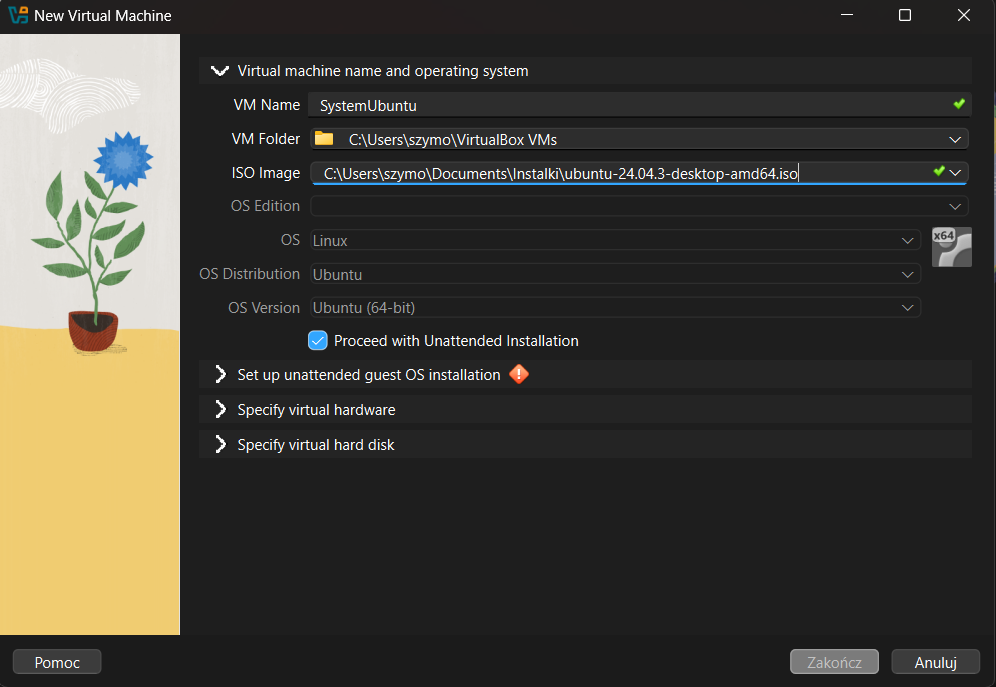
\includegraphics[width=0.7\textwidth]{screenshots/install02.png}
\end{figure}
\begin{itemize}
	\item W polu \texttt{'VM Name'} wpisz nazwę swojej Maszyny Wirtualnej.
	\item Pole \texttt{'VM Folder'} zawiera folder, w którym znajduje się twoja Maszyna Wirtualna, zaleca się zostawić domyślną opcję.
	\item W polu \texttt{'ISO Image'} wybierz folder, w którym znajduje pobrany wcześniej plik z systemem Ubuntu. Plik powinien być w formacie \textbf{.iso}
\end{itemize}

Teraz przejdź do zakładki \texttt{'Set up unattented guest OS installation'}.
\begin{figure}[H]
\centering
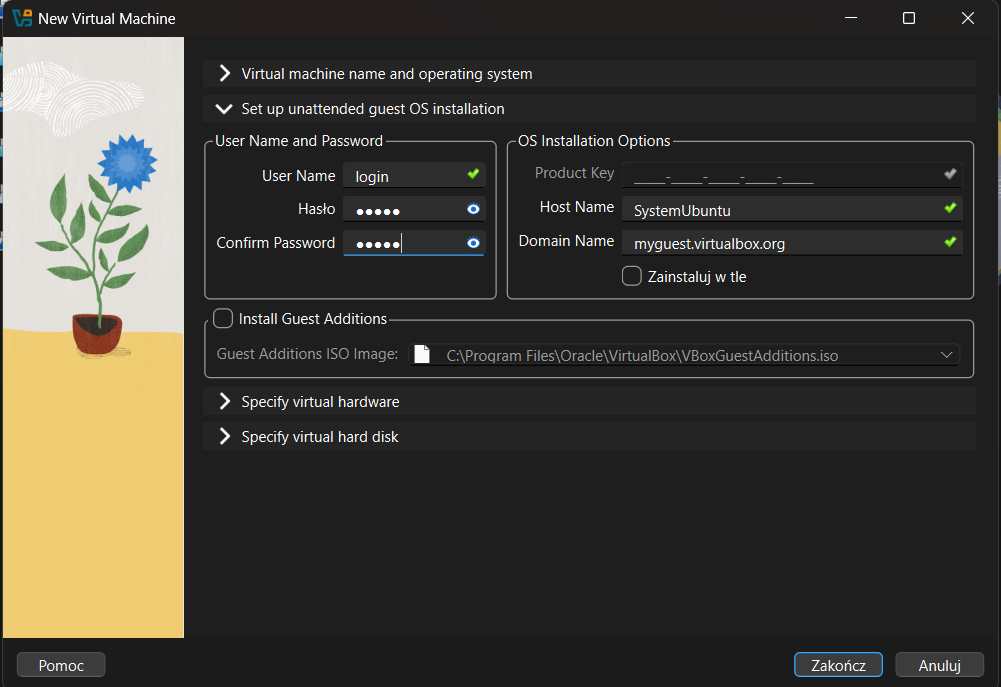
\includegraphics[width=0.7\textwidth]{screenshots/install03.png}
\end{figure}
\begin{itemize}
	\item W polu \texttt{'User Name'} wpisz nazwę użytkownika, czyli login do konta na Maszynie Wirtualnej.
	\item W polach \texttt{'Hasło'} oraz \texttt{'Confirm Password'} wpisz hasło do konta.
	\item W polach \texttt{'Host Name'} oraz \texttt{'Domain Name'} zostaw domyślne opcje.
\end{itemize}

Następnie przejdź do zakładki \texttt{'Specify Virtual Hardware'}.
\begin{figure}[H]
\centering
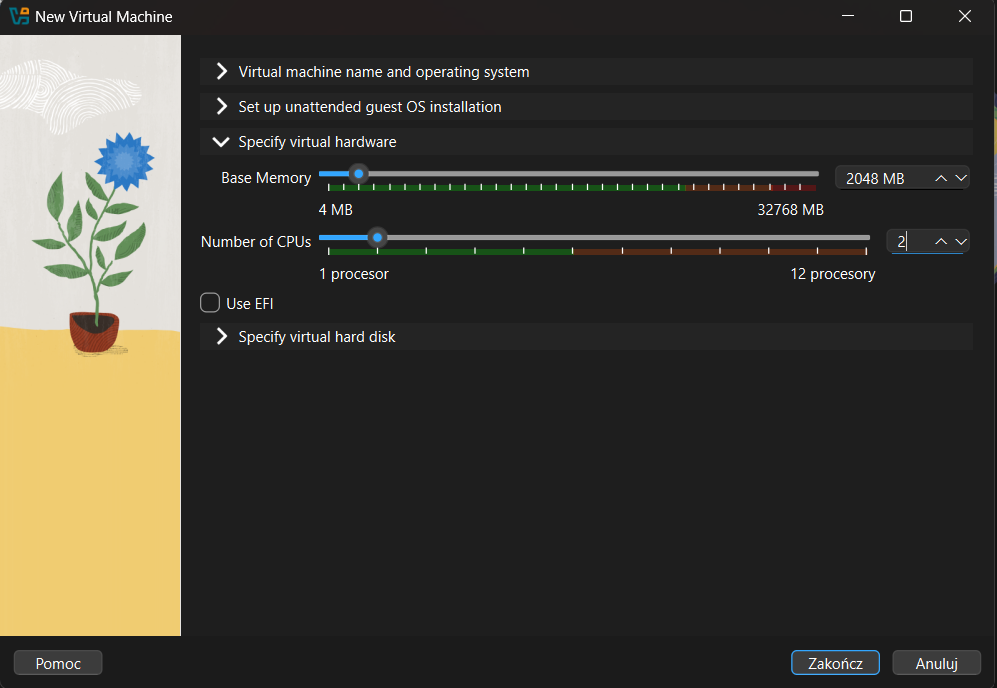
\includegraphics[width=0.7\textwidth]{screenshots/install04.png}
\end{figure}
\begin{itemize}
	\item W \texttt{'Base Memory'} ustal ilość pamięci przeznaczoną na Maszynę Wirtualną. Zalecane jest 4096MB (4GB), jednak minimalna ilość to 2048MB (2GB).
	\item W  \texttt{'Number of CPUs'} ustal ilość procesorów przeznaczonych na Maszynę Wirtualną. Zaleca się ustawić 2 procesory.
\end{itemize}

Na koniec przejdź do zakładki \texttt{'Specify Virtual Disk'}.
\begin{figure}[H]
\centering
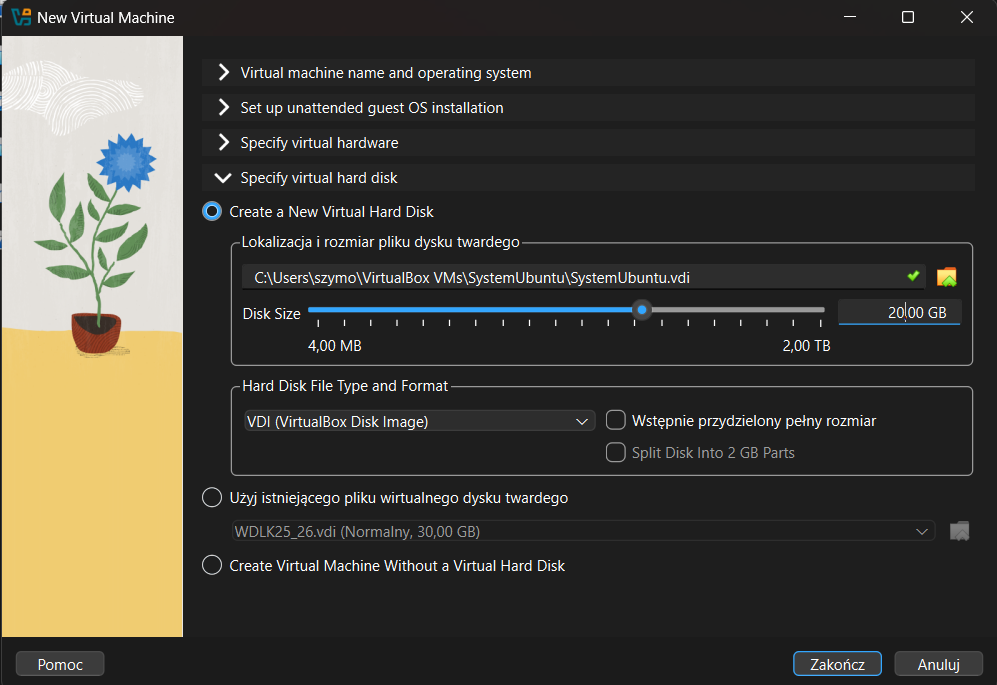
\includegraphics[width=0.7\textwidth]{screenshots/install05.png}
\end{figure}
\begin{itemize}
	\item Tutaj możesz ustalić ilość miejsca na wirtualnym dysku. Zaleca się ustawić około 20GB.
\end{itemize}
Po skończeniu ustawiania maszyny kliknij \texttt{Zakończ}.

\subsection{Konfiguracja Maszyny Wirtualnej}
Twoja Maszyna powinna od razu samoczynnie się włączyć, jednak jeśli tak się nie stanie, naciśnij zielony przycisk \texttt{Uruchom} na górze aplikacji \textit{(na tym zdjęciu w miejscu tego przycisku znajduje się przycisk \texttt{Pokaż})}.
\begin{figure}[H]
\centering
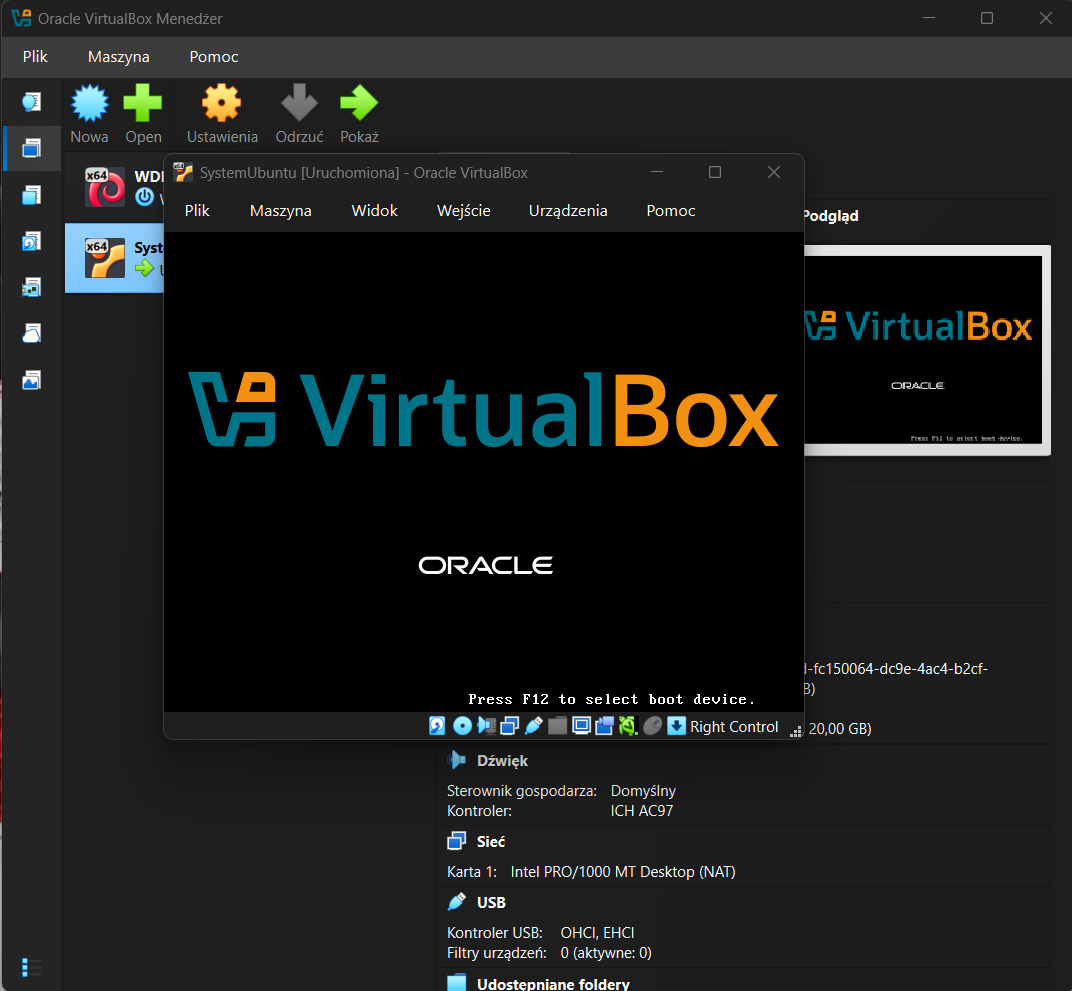
\includegraphics[width=0.5\textwidth]{screenshots/install06.png}
\end{figure}

Po chwili na oknie z Maszyną Wirtualną powinien pojawić się taki komunikat:
\begin{figure}[H]
\centering
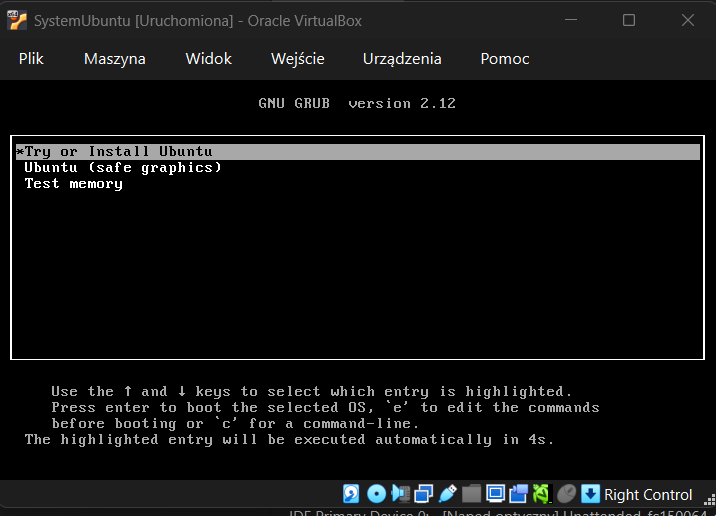
\includegraphics[width=0.7\textwidth]{screenshots/install07.png}
\end{figure}
Poruszając się strzałkami, zaznacz opcję \texttt{Try or Tnstall Ubuntu}.
Następnie system powinien zacząć się instalować i po chwili uruchomić.

\begin{figure}[H]
\centering
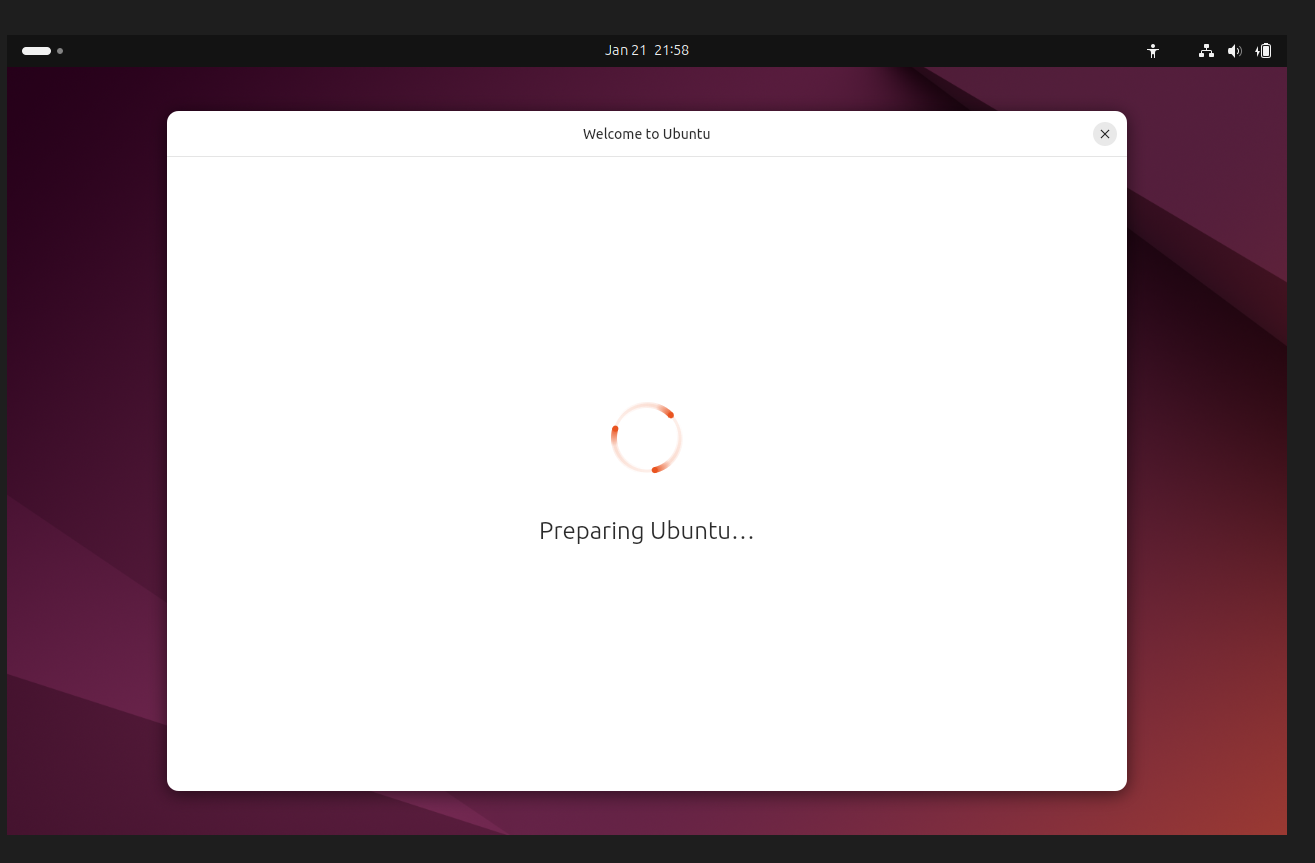
\includegraphics[width=0.6\textwidth]{screenshots/install08.png}
\vspace{1\baselineskip}
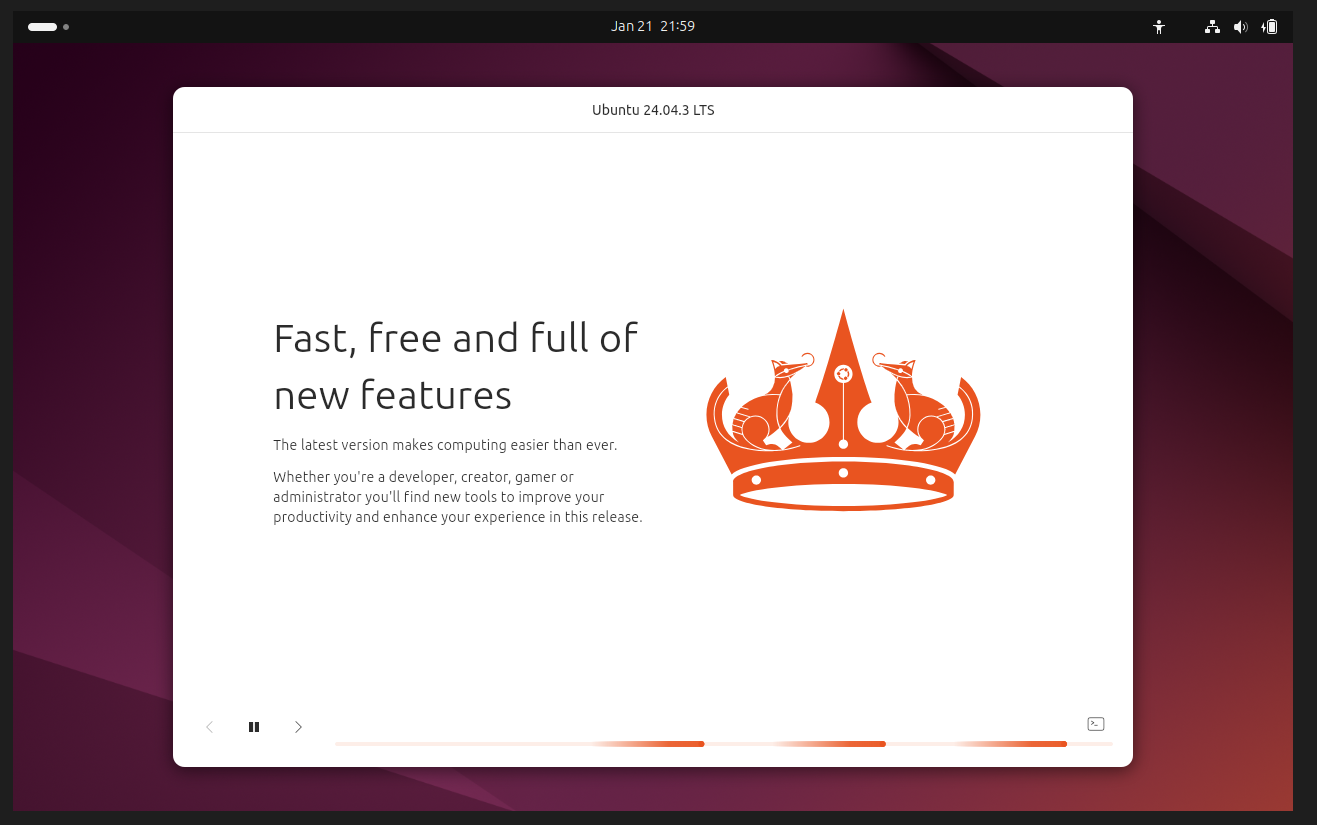
\includegraphics[width=0.6\textwidth]{screenshots/install09.png}
\end{figure}
\newpage
Po kilku minutach system powinien się zrestartować i pokazać ekran logowania:
\begin{figure}[H]
\centering
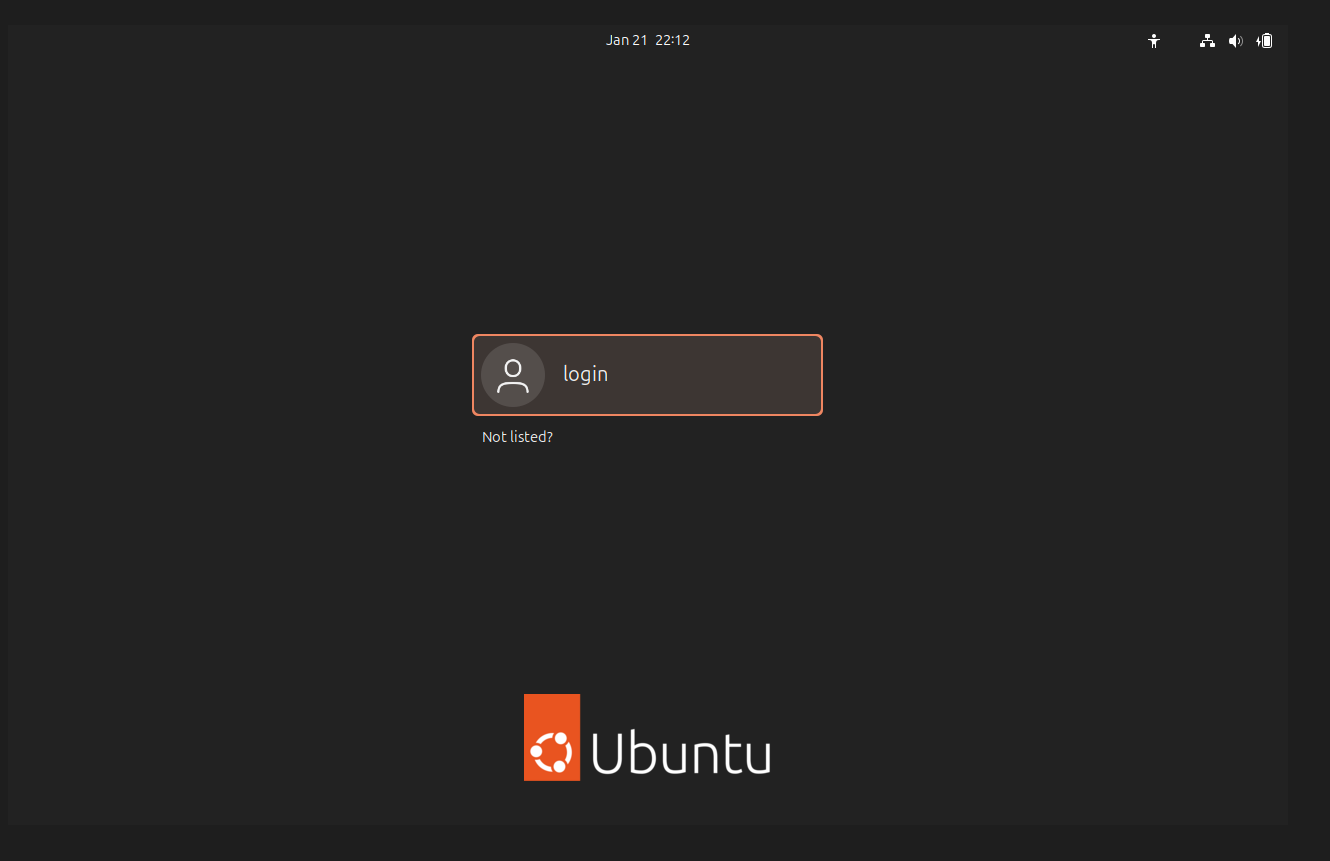
\includegraphics[width=0.7\textwidth]{screenshots/install10.png}
\end{figure}
Kliknij w kafelek ze swoją nazwą użytkownika, którą wpisywaliśmy przy stawianiu Maszyny, i wpisz hasło, żeby się zalogować.
\begin{figure}[H]
\centering
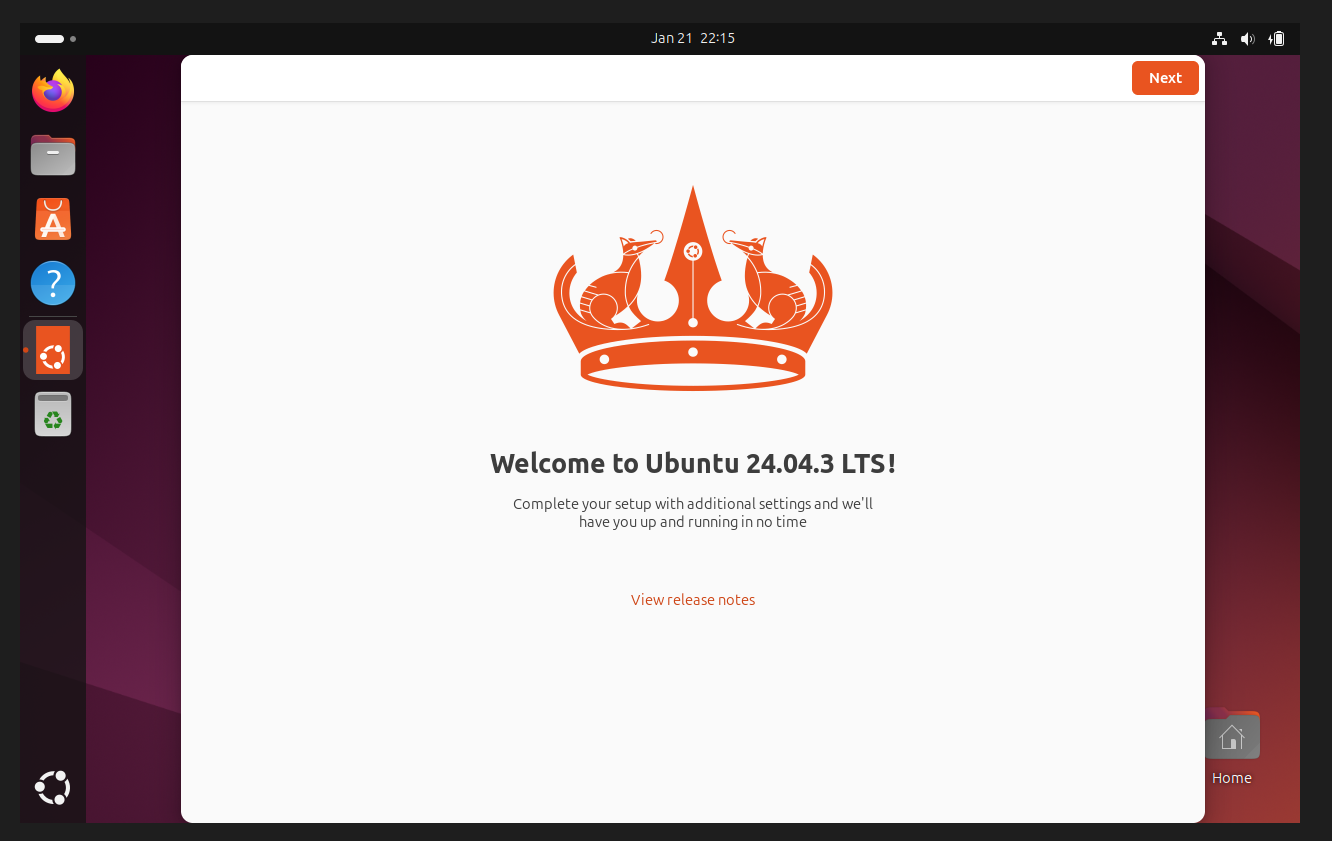
\includegraphics[width=0.7\textwidth]{screenshots/install11.png}
\end{figure}

Żeby pokazać lub schować pasek boczny naciśnij \texttt{przycisk Windows/Option}.

\vspace{2\baselineskip}
Brawo! Udało ci się zainstalować i skonfigurować Maszynę Wirtualną z systemem Ubuntu :D

\end{document}
